\subsection{Berechnung der Diskreten Fouriertransformation mittels FFT}
Die Mathematiker Cooley und Tukey haben einen Algorithmus entwickelt, mit dem sich die \gls{dft} mit vergleichsweise wenig Multiplikationen
und somit deutlich schneller als bei der allgemeinen \gls{dft} berechnen lässt. Sie machen sich in erster Linie zu nutze, dass sich eine DFT
in kleinere DFTs aufspalten lässt, welche entsprechend weniger Elemente und Koeffizienten haben. Aus Gleichung (\ref{eq:Twiddlefaktorenberechnung}) ist 
bekannt, dass die Variablen der Twiddlefaktorberechnung die Indizes der Eingangs- sowie Ausgangsvektoren sind. Hieraus lässt sich bereits erkennen, dass
die gesamte Twiddlefaktormatrix N verschiedene komplexe Werte enthält. Dies wird auch aus Abbildung (\ref{pic:Einheitskreis_Faktoren}) aus Abschnitt 
(\ref{sec:AnalyseBewertungTwiddlefaktornMatrizen}) am Beispiel für N=8 ersichtlich. Darüber hinaus lässt sich erkennen, dass die komplexen Zeiger den Einheitskreis 
in N Bereiche mit einem Winkel von $\frac{2 \pi}{N}$ unterteilen. Bekannt ist ebenfalls, dass der erste Wert immer die $1$ ist.
Daraus ergibt sich bei einer DFT mit 2 Eingangswerten die Twiddlefaktoren $1$ und $-1$, sodass eine Multiplikation wegfällt. Ähnlich verhält es sich mit der zweiten Stufe.
Hier ergeben sich die Werte $1, -j, -1, j$, was ebenfalls bedeutet, dass keine Multiplikation erfolgen muss. Tatsächlich müssen hier bei $j und -j$ nicht einmal eine
Additionen durchgeführt werden, da die Zahlen um einen Imaginärteil ergänzt werden. Dies hat jedoch zur Folge, dass in der dritten Stufe ein Teil der Berechnungen bedeutend
aufwändiger werden. 


aus  Darüber hinaus sind die Werte der 

Es ist erforderlich, dass hierfür die Werte im Eingangsvektor in die umgekehrte Bitreihenfolge getauscht werden. Dies geschieht nach dem Muster, dass die Indizes der Eingangswerte, wie
üblich bei 0 beginnend, binär dargestellt werden. Nun wird die Reihenfolge der Bits getauscht. Auf diese Weise tauschen bei einem 8-Bit Vektor die
Elemente 2 und 5 sowie 4 und 7 ihre Position.


\begin{figure}[htbp]
 \centering
 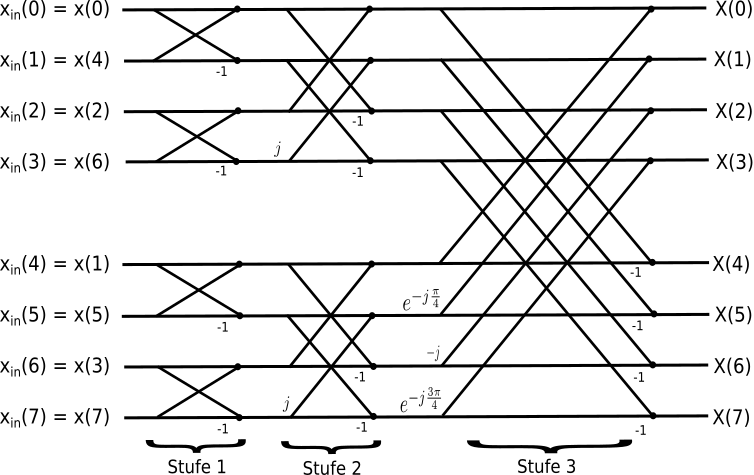
\includegraphics[width=0.7\textwidth]{img/Butterfly.png}
 \caption{8x8 Butterfly}
 \label{pic:Butterfly}
\end{figure}


Die Stufen 1 bis 3 in Abbildung (\ref{pic:Butterfly}) stellen 